\section{Preamble}
In this part of this work we define some notations and declare definitions which we will use.
In addition, some former mentioned aspects are being formalized.

Nodes which are contained in a graph are denoted in lower case arabic letters and upper case arabic letters are complete graphs.
A Graph consists of a set of nodes and a set of edges which connect nodes.
Let $\bigcirc{abc} $ be a circle with $a, b, c $ on its border.
%The circle with center $o $ is denoted by $(o) $.
%$\triangle{abc} $ is the triangle with corners $a,b $ and $c $.

Furthermore, we assume that there are no four points in any graph which are co-circular since the Delaunay Triangulation is in this case not unique anymore.
This leads to unnecessary case differentiation.

The Unit Disk Graph of a node set $s $ is denoted as $U_s $ or as $U $ if any node set can be used.
This graph contains all nodes of node set $s $ and connects two nodes if and only if their distance between each other is at most $1 $.
In addition, we will make use of the so called \emph{Gabriel Graph}, denoted as $GG $. 
It is the graph which contains all nodes of a supergraph $U $ and it contains an edge $uv \in U $ if and only if the Gabriel circle of $uv $ contains no other node.
The Gabriel circle of an edge $uv $ is denoted as $disk(u, v) $.
It is the circle with $u $ and $v $ on its border and with its center on line $uv $. 
In this work $U $ denotes the unit disk graph with unit disk radius $R = 1 $.

Another important graph in order to follow this work is the Partial Delaunay Triangulation (PDT)  \cite{pdt}. It is a planar, t-spanner of the Unit Disk Graph (refer to \ref{PDT_section}).

The following abbreviations are used throughout this work and introduced here.
\emph{Ready To Send (RTS)} and \emph{Clear To Send (CTS)} describe the process of a node pair to interchange messages while starting the desired topology control, namely PDT and RMYS.

Topology controls are algorithms which create a subgraph of a graph with specific properties.
Currently known topology controls can be divided into beacon and beaconless approaches.
In a topology control which uses beacons information is gathered periodically and possibly unnecessary information is interchanged which leads to a message overhead.
In this work a reactive algorithm is proposed and here, this means that the topology control does not use any beacons and no neighborhood information are available before the algorithms execution.




\subsection{Partial Delaunay Triangulation}
\label{PDT_section}
The Partial Delaunay Triangulation produces a connected, planar, t-spanner of any connected graph in a reactive approach.
No node needs to know its neighborhood.
In this part we will see an example of the reactive construction of $PDT $.
First, we define the Partial Delaunay Triangulation as follows:
\begin{definition}
\label{pdt-def}
An edge $uv \in U $ is in $PDT(U_s) $ if either 
\begin{enumerate}
\renewcommand{\labelenumi}{(\roman{enumi})}
 \item $uv \in GG $
 \item or $\exists{w} \in U : $ maximizes $\angle{uwv} $, $\bigcirc{uwv}  \backslash \{u, v, w\} = \emptyset $ and $\sin{\angle{uwv}} \geq\frac{|uv|}{R} $, with $R>0 $ being the unit disk radius.
\end{enumerate} 
\end{definition}

The $rPDT $ algorithm taken from chapter 3 of \cite{Benter2013} is presented briefly in the following (note that the original PDT definition is from \cite{pdt}):
\algrenewcommand\algorithmicprocedure{\textbf{}}
\begin{algorithm}\small
\caption{Partial Delaunay Triangulation}\label{pdt_alg}
\begin{algorithmic}[1]
\Statex \textbf{Input:} any node $u $ of a connected graph $G $
\Statex \textbf{Output:} planar, connected view on neighbors of $u $

\Statex
\State $u $ broadcasts a RTS including its position.
\State All nodes which overhear that message set a timer relative to the Euclidean distance to $u $ such that the closest node has the shortest timer.
\State As soon as a timer expires the corresponding node sends a CTS including its position.
\State If a node $v $ overhears a CTS from node $t $ it checks whether or not $uv $ violates certain geometric conditions which correspond to the conditions in definition \ref{pdt-def}.
If it does, $v $ cancels its timer and remains silent.


\end{algorithmic}
\end{algorithm}

%The former mentioned GPDT (generalized Partial Delaunay Triangulation) criteria is defined in \cite{Benter2013} as the following:
%\begin{definition}
%Let edge $uv \in U$.
%$uv \in GPDT $ if and only if the following is true for all nodes $w \in disk(u,v) $:
%\begin{enumerate}
%\item there is no node $x \in \bigcirc{u,v,w}$ $\cap $
%\end{enumerate}
%\end{definition}

\begin{figure}[p]
\centering
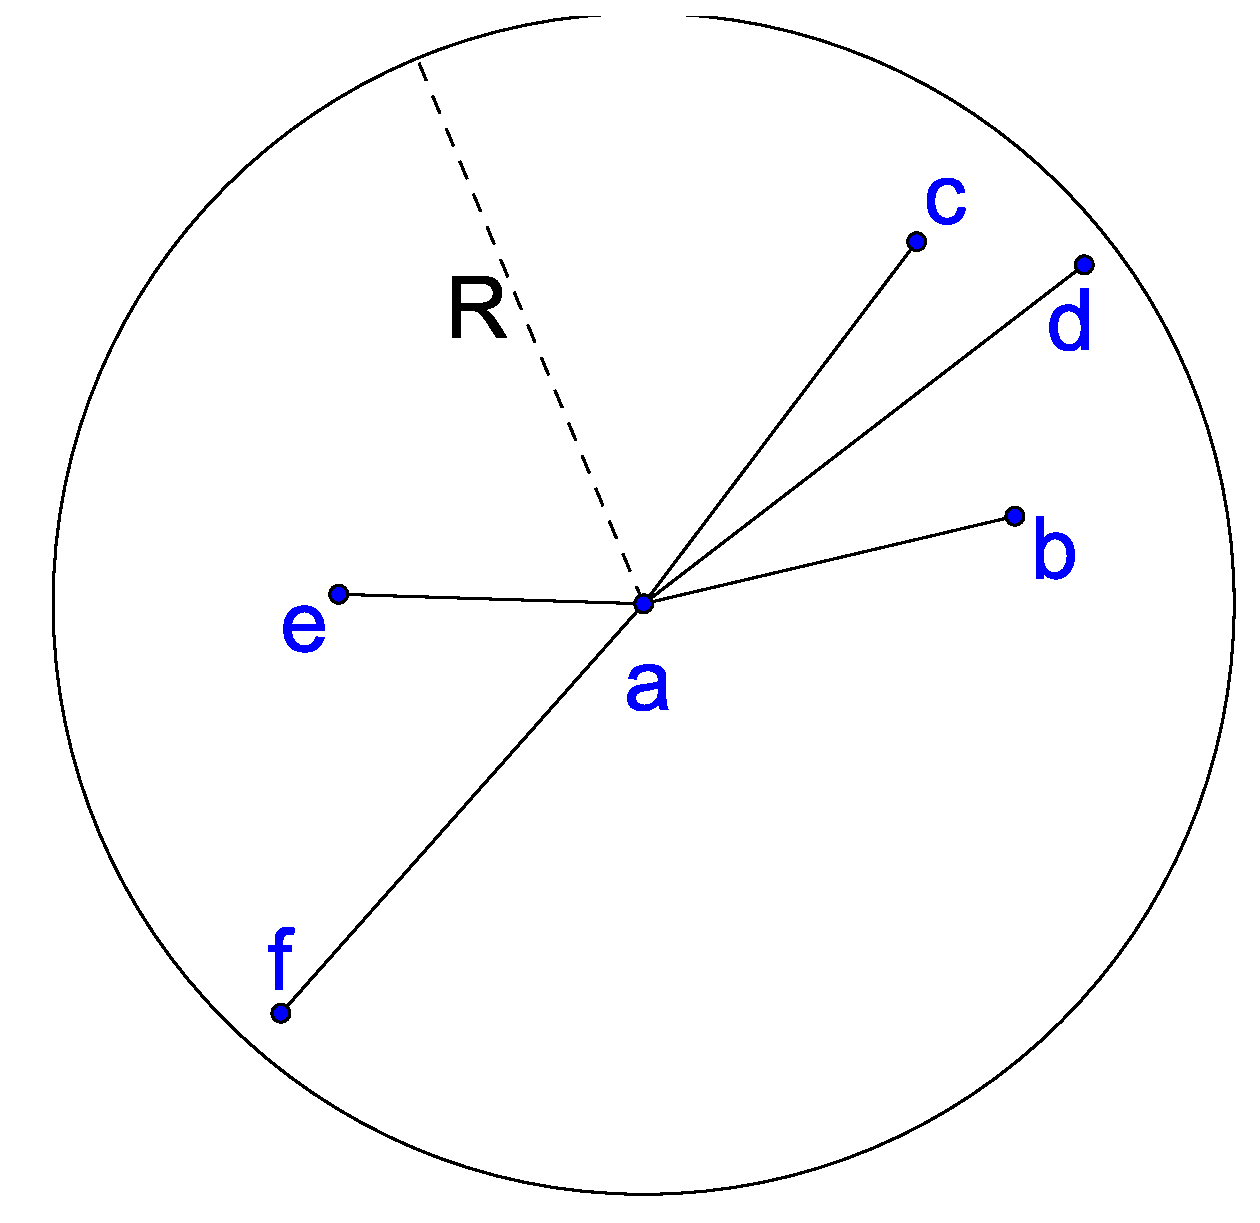
\includegraphics[width=0.35\linewidth]{eps/PDT_1.eps}
\caption{An example graph with unit disk radius $R $ with all edges drawn which are incident on $a $.}
\label{fig:PDT_1}
\end{figure}
Consider the graph in figure \ref{fig:PDT_1}.
We will use it as an example for the application of rPDT.
First, node $a $ sends a RTS and all other nodes set a timer relative to the Euclidean distance to $a $.
Since node $e $ is the closest to $a $ and therefore, there cannot be another node in $disk(a,e) $, its timer fires first and sends a CTS.
$f $ overhears that CTS and checks whether or not $e \in disk(a,f) $.
Since $e \in disk(a,f) $ is indeed true, $af \notin GG $.
However, $af $ is still a PDT edge.
The current angle maximizing node $e $ for edge $af $ ($\angle{aef} $) satisfies the conditions that first, $\bigcirc{aef} $ is empty and second, that $\sin{\angle{aef}} \geq\frac{|af|}{R} $ which means that $\bigcirc{aef} $ does not overlap the unit disk of $a $ and hence, $a $ can decide with only one-hop neighborhood information available that $af \in PDT(U)$.
These steps are visualized in figure \ref{fig:PDT_2}.
\begin{figure}[p]
\centering
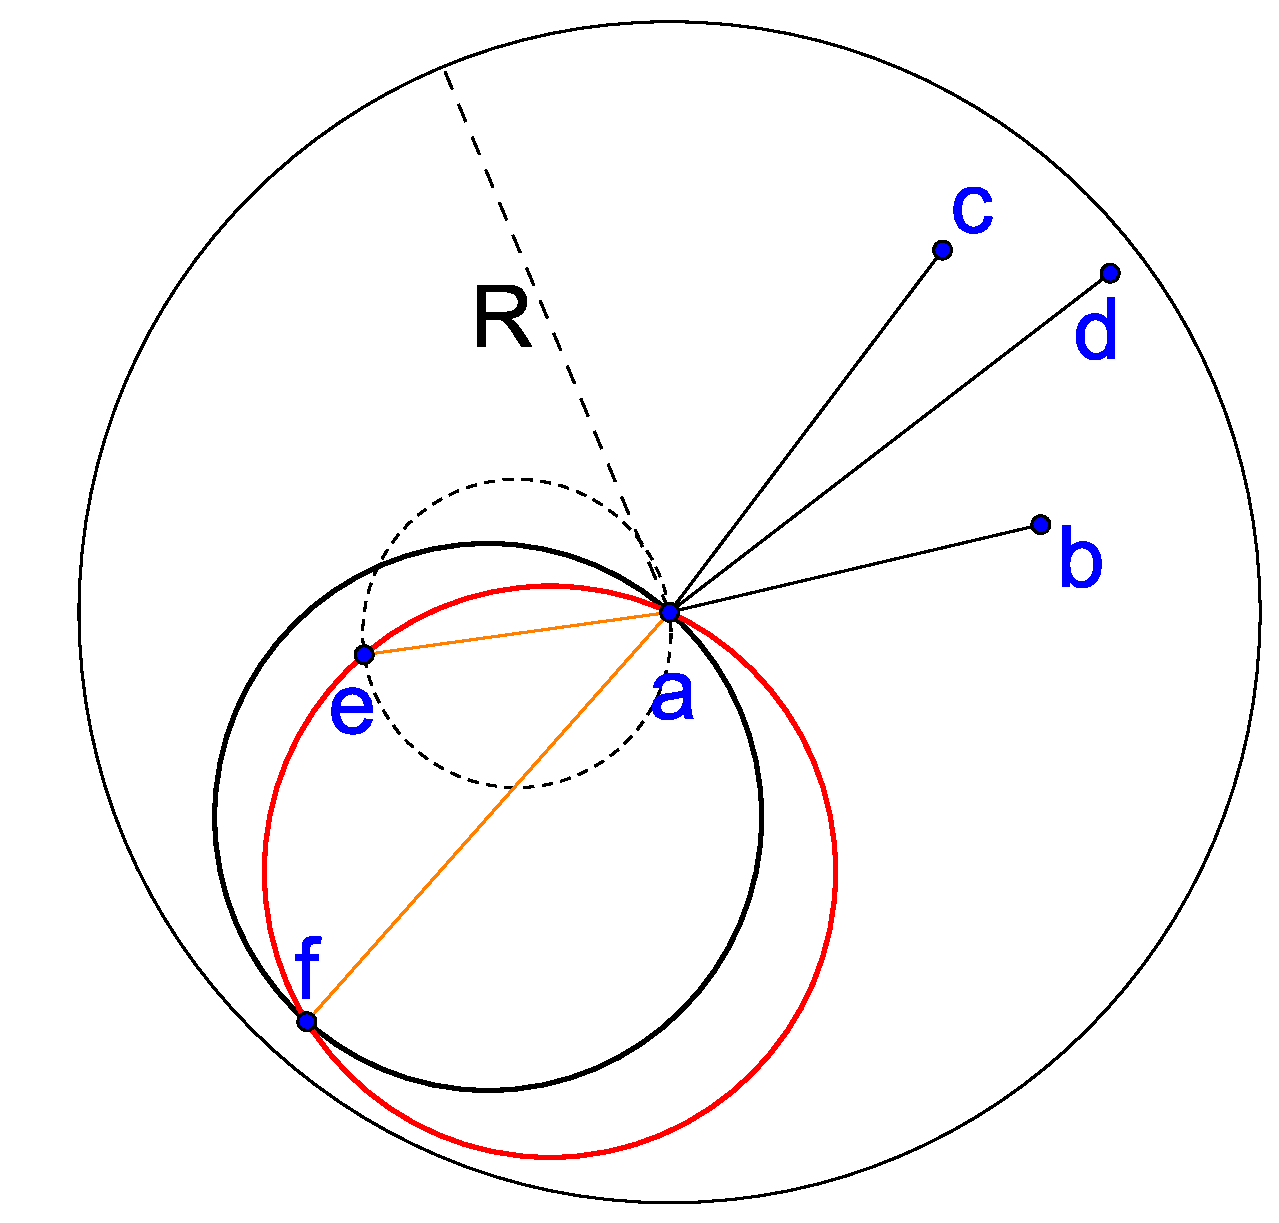
\includegraphics[width=0.35\linewidth]{eps/PDT_2.eps}
\caption{The dashed Gabriel Circle of edge $ae $ and $\bigcirc{aef} $ proof that both edges $ae $ and $af $ are PDT-edges.}
\label{fig:PDT_2}
\end{figure}
The subsequent steps are that $b $ and then $c $ sends a CTS, since both edges are Gabriel edges (refer to figure \ref{fig:PDT_3}).
First, $d $ overhears $b $' CTS, calculates that $b \in disk(a,d) $ and finally that $\bigcirc{abd} $ is empty.
From that point $d $ did not stop its timer yet.
When the CTS from node $c $ arrives at $d $, $\bigcirc{abd} $ is not empty anymore and there cannot be another circle which is empty.
$d $ cancels its timer since it is no PDT neighbor.
Figure \ref{fig:PDT_3} shows also the final edge selection of node $a $ after execution of rPDT.
\begin{figure}[p]
\centering
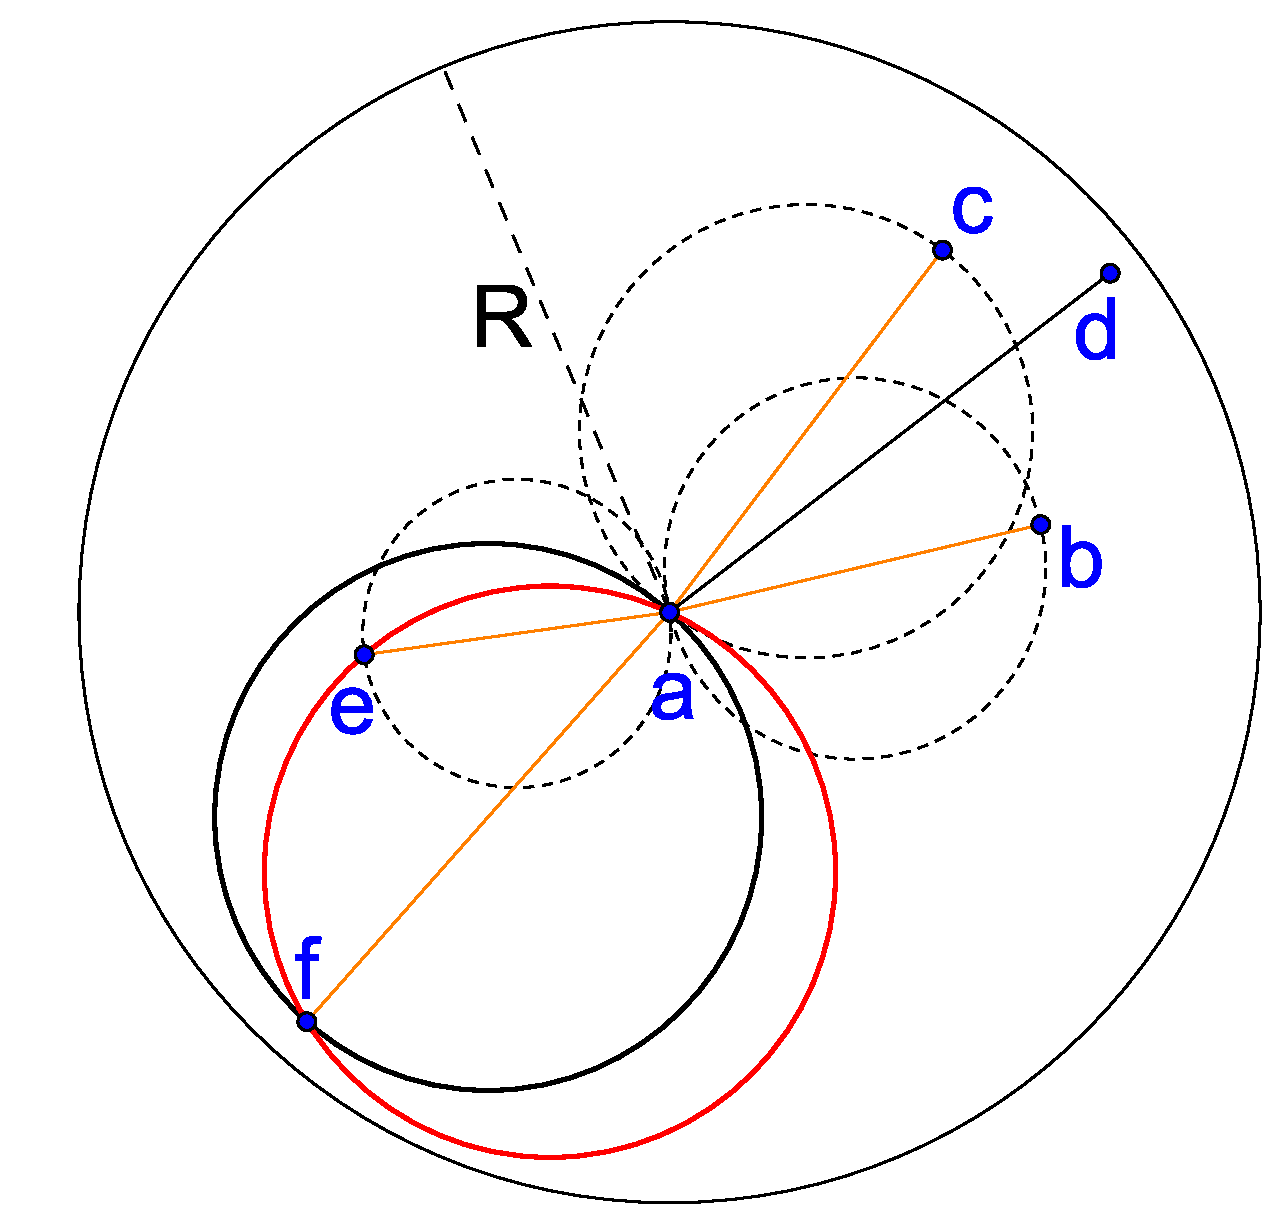
\includegraphics[width=0.35\linewidth]{eps/PDT_3.eps}
\caption{All endpoints of orange edges are PDT neighbors of $a $. Dotted circles are Gabriel circles and the red circle proofs that $af $ is a PDT edge.}
\label{fig:PDT_3}
\end{figure}